\documentclass[sigplan,10pt,review]{acmart}
\settopmatter{printfolios=true,printccs=false,printacmref=false}
\citestyle{acmnumeric}
\setcopyright{none}
\acmConference{McGill HLS Project Report}{}{Montreal, Canada}
\acmYear{2026}
\acmDOI{}
\acmISBN{}

\usepackage{booktabs}
\usepackage{graphicx}
\usepackage{tikz}
\usetikzlibrary{arrows.meta,positioning}

\begin{document}

\title{Constraint-Aware E-Graph Optimization for High-Level Synthesis}
\author{Ali Seifeldin}
\affiliation{%
  \institution{McGill University}
  \city{Montreal}
  \country{Canada}
}
\date{April 4, 2026}

\begin{abstract}
SEER shows that equality saturation can support high-level synthesis (HLS), but generating many equivalent datapaths is only the first step. A designer still has to choose one implementation under area, latency, and resource constraints. This report studies that selection problem with a datapath-only prototype for constraint-aware extraction. The prototype is implemented in Rust with \texttt{egg}. It saturates arithmetic graphs once, keeps a bounded frontier of candidates, and answers weighted, constrained, and exact area--latency Pareto queries with one shared analytical model. The model tracks area, latency, DSP/LUT usage, and a normalized power proxy. On six arithmetic kernels, default weighted extraction reduces analytical area by 40.9\% on average, but worsens analytical latency by 13.7\% and normalized power proxy by 44.6\% because it often replaces DSP-intended implementations with LUT-heavy alternatives. Latency-optimal extraction improves analytical latency by 41.7\% on average, and constrained queries often select implementations that differ from the weighted point. Generated RTL variants are checked with ModelSim against independent benchmark formulas. Quartus fit/STA also shows that multiplier-heavy variants can trade fitted DSP blocks for ALMs while changing reported Fmax. This FPGA evidence is useful but limited: it supports resource steering for generated RTL, not global FPGA optimality or a calibrated power model. The main result is that SEER-style e-graph optimization needs explicit extraction objectives and budgets to turn equivalent datapaths into useful design choices.
\end{abstract}

\maketitle
\begin{center}
\small April 4, 2026
\end{center}

\section{Introduction}
High-level synthesis raises the abstraction level of hardware design, but arithmetic kernels remain highly sensitive to expression structure, operator binding, and resource allocation \cite{cong2011hls}. SEER shows that equality saturation is attractive in this setting because an e-graph can retain many equivalent implementations and avoid phase-ordering mistakes during optimization \cite{cheng2024seer}. The next problem is selection. Once many equivalent datapaths exist, an HLS flow still needs to choose the minimum-latency implementation under an area budget, the minimum-area implementation under a latency budget, or a feasible implementation under explicit DSP/LUT limits. An e-graph alone does not answer those budgeted design questions.

This project studies that missing extraction step. The goal is not to reproduce the full SEER stack or build a complete HLS compiler. Instead, the prototype focuses on datapath selection: it represents kernels directly as arithmetic graphs, rewrites them with equality saturation, and asks how different objectives and hard budgets change the selected implementation under one analytical cost model.

The project has four concrete contributions:
\begin{itemize}
\item a datapath-only SEER-style optimizer that saturates each benchmark once and reuses a bounded retained frontier for later queries;
\item a shared analytical cost model over area, latency, DSP/LUT usage, and a normalized power proxy;
\item extraction modes for weighted selection, constrained optimization, infeasibility reporting, and Pareto tradeoff exploration;
\item validation that combines analytical benchmark results, generated RTL functional simulation, and narrow Quartus resource-steering evidence.
\end{itemize}

The code, scripts, and generated artifacts are available in the project repository \cite{seeroptimizerrepo}.

The evaluation asks four matching questions: is weighted extraction enough, do constraints select different points, do hard budgets expose infeasible cases, and does generated RTL preserve behavior while steering fitted resources? The core claim is straightforward: for SEER-style equality saturation in HLS, generating equivalent implementations is not enough.

A small example shows why selection matters. Throughout the report, $A/L/P/D/U$ denotes analytical area, analytical latency, normalized power proxy, DSP count, and LUT count. On \texttt{fir8}, the retained frontier contains a low-area weighted point with metrics 25/18/33/0/41, a low-latency point with metrics 38/9/31/10/10, and a lower power-proxy point with metrics 33/16/21/4/9. All three implementations are algebraically equivalent, but they answer different model-level design questions. The project is therefore not simply to generate more equivalent expressions than SEER; it is to make those expressions selectable under explicit goals and budgets.

\section{Related Work}
\texttt{egg} makes equality saturation practical by combining efficient e-matching, rebuilding, and extraction with a usable systems interface \cite{willsey2021egg}. That infrastructure is the mechanism behind this project: rewrites create a space of equivalent arithmetic implementations, and extraction selects one of them.

SEER is the closest HLS reference \cite{cheng2024seer}. It shows that e-graphs can organize optimization in an HLS-relevant compiler flow, but it does not focus on constrained selection as the main evaluation target. This project asks the narrower follow-up question: once the e-graph exists, how should an HLS tool extract implementations under explicit budgets and competing objectives?

Datapath-oriented work by Coward et al.\ is the closest extraction-focused comparison. Their systems show that e-graphs can recover strong arithmetic datapath optimizations and then extend that line with constraint-aware extraction and power-aware rewriting \cite{coward2022automatic,coward2023constraint,coward2024power}. This project is smaller in scope, but follows the same basic idea: explore arithmetic equivalences once, then filter them with explicit objectives and budgets instead of one scalar heuristic. Relative to SEER, this project contributes constrained extraction and tradeoff analysis, but not an MLIR/CIRCT extension, full HLS frontend, or synthesis-calibrated hardware model.

\section{Approach and System Design}
Figure~\ref{fig:workflow} gives the end-to-end project flow. Read the boxes as data artifacts that the project creates or consumes, and read the arrows as the tools or actions that transform them. The top row is the main optimizer and reporting path; the lower branches show the exploratory C++/\texttt{i++} path, the ModelSim functional-test path, and the Quartus fit/STA path. The subsections then define the IR, retained frontier, extraction modes, and analytical model used by the evaluation.
\begin{figure*}[t!]
\centering
\resizebox{\textwidth}{!}{%
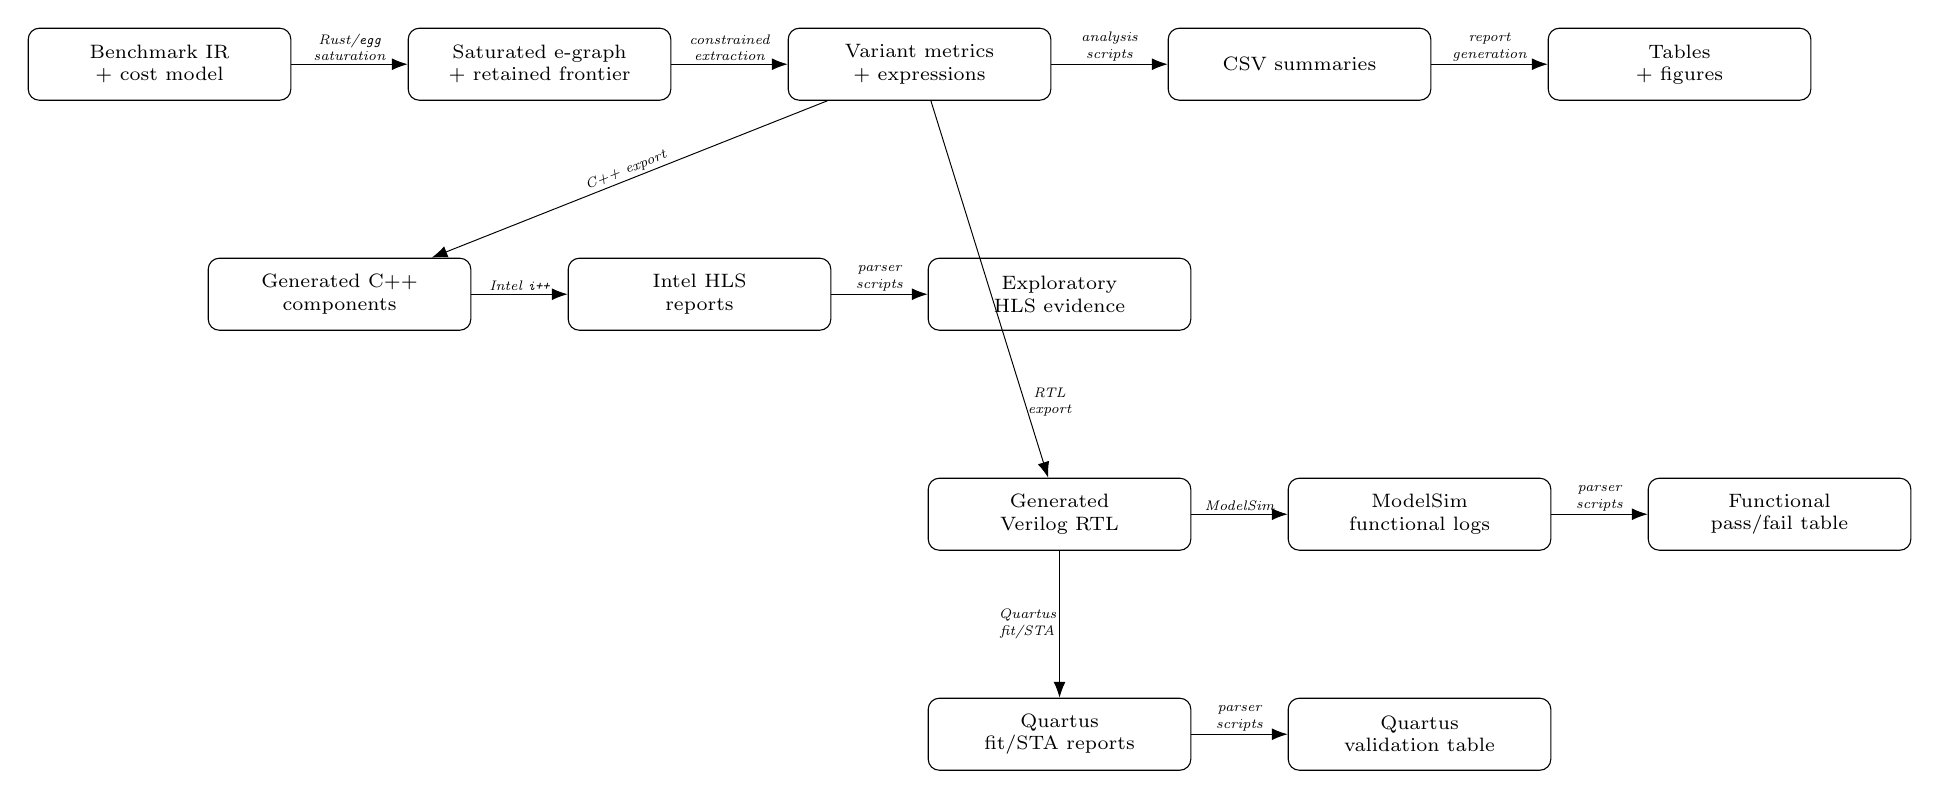
\begin{tikzpicture}[
  x=1in,
  y=1in,
  artifact/.style={
    draw,
    rounded corners,
    align=center,
    inner sep=3pt,
    minimum height=0.36in,
    text width=1.23in,
    font=\scriptsize
  },
  action/.style={font=\tiny\itshape, align=center, inner sep=1pt},
  arrow/.style={-{Latex[length=2mm]}, line width=0.35pt}
]
\node[artifact] (ir) at (0,0) {Benchmark IR\\+ cost model};
\node[artifact] (eg) at (1.9,0) {Saturated e-graph\\+ retained frontier};
\node[artifact] (variants) at (3.8,0) {Variant metrics\\+ expressions};
\node[artifact] (csv) at (5.7,0) {CSV summaries};
\node[artifact] (paper) at (7.6,0) {Tables\\+ figures};

\node[artifact] (cpp) at (0.9,-1.15) {Generated C++\\components};
\node[artifact] (hls) at (2.7,-1.15) {Intel HLS\\reports};
\node[artifact] (hlsout) at (4.5,-1.15) {Exploratory\\HLS evidence};

\node[artifact] (rtl) at (4.5,-2.25) {Generated\\Verilog RTL};
\node[artifact] (sim) at (6.3,-2.25) {ModelSim\\functional logs};
\node[artifact] (funout) at (8.1,-2.25) {Functional\\pass/fail table};

\node[artifact] (fit) at (4.5,-3.35) {Quartus\\fit/STA reports};
\node[artifact] (qout) at (6.3,-3.35) {Quartus\\validation table};

\draw[arrow] (ir) -- node[action, above] {Rust/\texttt{egg}\\saturation} (eg);
\draw[arrow] (eg) -- node[action, above] {constrained\\extraction} (variants);
\draw[arrow] (variants) -- node[action, above] {analysis\\scripts} (csv);
\draw[arrow] (csv) -- node[action, above] {report\\generation} (paper);

\draw[arrow] (variants) -- node[action, above, sloped] {C++ export} (cpp);
\draw[arrow] (cpp) -- node[action, above] {Intel \texttt{i++}} (hls);
\draw[arrow] (hls) -- node[action, above] {parser\\scripts} (hlsout);

\draw[arrow] (variants) -- node[action, right, pos=0.80] {RTL\\export} (rtl);
\draw[arrow] (rtl) -- node[action, above] {ModelSim} (sim);
\draw[arrow] (sim) -- node[action, above] {parser\\scripts} (funout);

\draw[arrow] (rtl) -- node[action, left] {Quartus\\fit/STA} (fit);
\draw[arrow] (fit) -- node[action, above] {parser\\scripts} (qout);
\end{tikzpicture}
}
\caption{End-to-end project flow. Boxes are data artifacts; arrows are tools or actions. The top row shows the optimizer and report-generation path. The lower branches show exploratory C++/\texttt{i++} HLS evidence, ModelSim functional checks, and Quartus DSP/ALM evidence.}
\label{fig:workflow}
\end{figure*}

\subsection{IR and Rewrite Space}
The IR contains \texttt{input}, \texttt{const}, \texttt{add}, \texttt{sub}, and \texttt{mul} nodes plus architecture-aware variants such as \texttt{add\_lut}, \texttt{add\_dsp}, \texttt{mul\_lut}, \texttt{mul\_dsp}, and \texttt{mac\_dsp}. Rewrites cover constant folding, neutral-element elimination, algebraic reassociation, and datapath mapping alternatives. Additions and subtractions may bind to LUT or DSP implementations; multiplications may bind to LUT or DSP variants; and multiply-accumulate structure can be recognized and replaced with a fused DSP MAC.

\subsection{Equality Saturation and Frontier Construction}
Each benchmark is serialized as a JSON arithmetic DAG, then saturated once in the Rust core using \texttt{egg}. The system computes a bounded deterministic frontier rather than retaining one extracted term per e-class. Child frontiers are combined bottom-up, candidates with identical metric vectors are deduplicated, dominated points are removed in five dimensions, and survivors are kept in lexicographic order with a 128-candidate cap per e-class and a 16-pass convergence limit. Equality saturation creates the design space once; later extraction queries reuse the retained frontier to answer multiple model-level design questions.

\subsection{Constraint-Aware Extraction}
Each candidate carries a metric vector $(A,L,P,D,U)$ for area, latency, normalized power proxy, DSP count, and LUT count. Weighted extraction provides a default scalar baseline via $\mathrm{score}(x)=w_aA(x)+w_lL(x)+w_pP(x)$, but the main interface is constrained extraction. The system can minimize latency under an area cap, minimize area under a latency cap, minimize latency under DSP or LUT budgets, and minimize the power proxy under a latency constraint. These modes correspond directly to the design questions that motivated the project: minimum modeled latency under an area budget, minimum modeled area under a latency budget, minimum modeled power proxy under a latency target, or feasibility under explicit resource ceilings.

\subsection{Pareto and Tradeoff Exploration}
The project also exposes the design space instead of only returning one answer. Exact Pareto extraction projects the retained candidate set onto area versus latency to produce a compact nondominated frontier. The reports then show where weighted, latency-optimal, and power-proxy choices sit relative to one another. This is the main difference from a pure SEER-style ``generate equivalences'' story: the user can inspect the tradeoff instead of accepting one extracted point with little context.

\subsection{Analytical Cost Model}
Metrics are analytical rather than synthesis-derived. Area, normalized power proxy, DSP count, and LUT count are additive over children plus the local operator cost; latency follows the longest dependency path plus local operator latency. Formally, for operation $o$ with children $c_i$, $A=\sum_i A(c_i)+A(o)$, $P=\sum_i P(c_i)+P(o)$, $D=\sum_i D(c_i)+D(o)$, $U=\sum_i U(c_i)+U(o)$, and $L=\max_i L(c_i)+L(o)$. The power proxy strengthens the constrained-extraction interface, but it is a secondary objective rather than a claim of device-accurate energy modeling. Table~\ref{tab:cost-model} gives the complete operation table used by both the Rust extractor and Python benchmark harness.

\begin{table}[t]
\caption{Complete operation costs from the shared analytical model.}
\label{tab:cost-model}
\centering
\footnotesize
\setlength{\tabcolsep}{3pt}
\begin{tabular}{lrrrrr}
\toprule
Op & Area & Lat. & Power & DSP & LUT \\
\midrule
\texttt{input} & 0 & 0 & 0 & 0 & 0 \\
\texttt{const} & 0 & 0 & 0 & 0 & 0 \\
\texttt{add} & 1 & 2 & 1 & 0 & 1 \\
\texttt{add\_lut} & 1 & 2 & 1 & 0 & 1 \\
\texttt{add\_dsp} & 2 & 1 & 2 & 1 & 0 \\
\texttt{sub} & 1 & 2 & 1 & 0 & 1 \\
\texttt{sub\_lut} & 1 & 2 & 1 & 0 & 1 \\
\texttt{sub\_dsp} & 2 & 1 & 2 & 1 & 0 \\
\texttt{mul} & 6 & 3 & 3 & 1 & 0 \\
\texttt{mul\_dsp} & 6 & 3 & 3 & 1 & 0 \\
\texttt{mul\_lut} & 4 & 6 & 6 & 0 & 8 \\
\texttt{mac\_dsp} & 7 & 3 & 4 & 1 & 0 \\
\bottomrule
\end{tabular}
\end{table}

\section{Implementation}
The optimizer core is implemented in Rust 2024 using \texttt{egg} 0.10 and \texttt{serde}/\texttt{serde\_json}. \texttt{ir.rs} defines the request/response schema, metric arithmetic, budget checks, and dominance relation. \texttt{optimizer.rs} converts the input DAG to an \texttt{egg} expression, runs equality saturation, constructs the bounded per-eclass frontier, and answers weighted, constrained, or Pareto queries from the retained root frontier. \texttt{main.rs} exposes single-query and batch JSON entry points.

In execution terms, the Rust path has three phases. First, equality saturation builds the shared equivalence space. Second, frontier extraction compresses that space into a bounded retained candidate set at the root e-class. Third, query-time selection filters that retained set by budgets and chooses the best feasible candidate for the requested objective. This decomposition matters because the first two phases are shared across all queries for one benchmark, while only the last phase changes when the user asks a different hardware question.

The Python harness builds benchmark graphs, computes baseline metrics from the shared cost model, invokes the Rust binary once per benchmark, and flattens results into CSV, HTML, and paper-ready figures. Batch mode keeps saturation and frontier construction shared across all queries for one benchmark; only the final selector differs between weighted, constrained, and Pareto extraction. As Figure~\ref{fig:workflow} shows, the project also generates C++ for an Intel \texttt{i++} path. That path is useful as an HLS frontend check, but direct Verilog is the main validation path because Intel HLS can legally remap equivalent C++ arithmetic to similar hardware.

\section{Experimental Setup}
The analytical evaluation runs on a MacBook Pro with an Apple M4 CPU and 16\,GB memory, using \texttt{rustc} 1.94.0, \texttt{cargo} 1.94.0, and Python 3.13.9. A follow-up pass uses generated RTL, ModelSim, and Quartus Prime Pro 19.2 on an Arria 10 target. Quartus is used only for fitted DSP/ALM/Fmax evidence; analytical area, analytical latency, and normalized power proxy remain the optimizer's objective metrics. The Intel \texttt{i++} reports are included only as exploratory evidence because most HLS estimates collapse distinct source variants to identical hardware estimates.

The benchmark suite contains six arithmetic kernels chosen to reflect the proposal's datapath focus: an 8-tap FIR accumulation (\texttt{fir8}), a 16-element dot product (\texttt{dot16}), two GEMM-style accumulations, a single \texttt{conv3x3} window, and a 5-point stencil (\texttt{stencil5}). These kernels are represented directly as arithmetic graphs, which keeps the experiment focused on extraction rather than parsing or frontend lowering.

\begin{table}[t]
\caption{Benchmark baselines and per-query hard-budget ceilings. Metrics use $A/L/P/D/U$ for area, latency, normalized power proxy, DSP count, and LUT count. The cap tuple lists the ceilings used by separate constrained queries: original area, latency, and power-proxy values; zero-DSP stress cap; and benchmark-specific LUT cap.}
\label{tab:benchmarks}
\centering
\footnotesize
\setlength{\tabcolsep}{3pt}
\resizebox{\columnwidth}{!}{%
\begin{tabular}{@{}l l c c c c@{}}
\toprule
Benchmark & Kernel & Mul/Add & Base A/L/P/D/U & Query caps A/L/P/D/U & Pareto \\
\midrule
\texttt{fir8} & 8-tap FIR & 8/7 & 55/17/31/8/7 & 55/17/31/0/7 & 10 \\
\texttt{dot16} & dot product & 16/15 & 111/33/63/16/15 & 111/33/63/0/15 & 16 \\
\texttt{gemm\_k8} & GEMM accum. & 8/7 & 55/17/31/8/7 & 55/17/31/0/7 & 11 \\
\texttt{gemm\_blocked\_k8} & blocked GEMM & 8/7 & 55/11/31/8/7 & 55/11/31/0/7 & 8 \\
\texttt{conv3x3} & conv. window & 9/8 & 62/19/35/9/8 & 62/19/35/0/8 & 10 \\
\texttt{stencil5} & stencil update & 5/4 & 34/11/19/5/4 & 34/11/19/0/4 & 8 \\
\bottomrule
\end{tabular}
}
\end{table}

Saturation limits are fixed to 12 iterations, 12{,}000 e-nodes, and 800\,ms per benchmark. For each benchmark, the harness executes default weighted extraction, unconstrained latency and power-proxy queries, four proposal-style constrained queries, a zero-DSP query, a LUT-capped query, and exact area--latency Pareto extraction. Because the evaluation is deterministic and analytical, one run per configuration is sufficient. The original graph is the baseline, default weighted extraction is the SEER-style single-answer comparison point, and the constrained modes test whether explicit extraction interfaces materially change the selected design.

The budget profiles are chosen to make the constrained queries interpretable against the original design rather than against an arbitrary external target. Table~\ref{tab:benchmarks} records these baseline ceilings explicitly. We write each constrained query as objective $|$ hard constraint. `min Lat $|$ Area cap' uses the original area as a hard ceiling and therefore asks whether latency can be improved without growing the implementation. `min Area $|$ Lat cap' and `min Power $|$ Lat cap' use the original latency as a ceiling and therefore ask whether the datapath can be compacted or reduce the normalized power proxy without slowing it down. `min Lat $|$ Power cap' uses the original power-proxy value as a ceiling and asks whether the same power-proxy class can support a lower-latency mapping. The remaining two profiles intentionally stress resource substitution: `min Lat $|$ DSP=0' forces a LUT-only implementation, while the benchmark-specific LUT caps expose whether a kernel can escape LUT-heavy weighted solutions at all.

\section{Evaluation}
The evaluation mirrors the four contributions: it checks the weighted baseline, constrained selection, infeasibility reporting, and generated RTL validation.
Across the suite, weighted extraction reduces analytical area by 40.9\% on average but regresses analytical latency by 13.7\% and normalized power proxy by 44.6\%. Latency-optimal extraction instead improves analytical latency by 41.7\% on average, while power-proxy-optimal extraction is conservative and improves the normalized power proxy by 7.8\%. These averages separate the roles of the modes: weighted extraction is primarily an area heuristic, latency-optimal extraction minimizes the model's latency metric, and power-proxy extraction is a secondary objective. The rest of the evaluation asks whether changing the selector changes the implementation qualitatively and whether infeasible cases line up with the intended resource restrictions.

\begin{table*}[t]
\caption{Cross-benchmark evidence for the constrained-extraction extension. Each result tuple is $A/L/P/D/U$, so the table reports total DSP and LUT use for the plotted weighted, latency-optimal, and power-proxy-optimal points.}
\label{tab:main-results}
\centering
\scriptsize
\setlength{\tabcolsep}{3pt}
\begin{tabular}{p{0.13\textwidth}p{0.15\textwidth}p{0.15\textwidth}p{0.15\textwidth}p{0.05\textwidth}p{0.25\textwidth}}
\toprule
Benchmark & Weighted A/L/P/D/U & Lat-opt A/L/P/D/U & P-proxy-opt A/L/P/D/U & Pareto & Infeasible query \\
\midrule
\texttt{fir8} & 25/18/33/0/41 & 38/9/31/10/10 & 33/16/21/4/9 & 10 & -- \\
\texttt{dot16} & 79/36/111/0/143 & 94/21/126/15/128 & 93/33/90/7/87 & 16 & min Lat $|$ Power cap; min Lat $|$ LUT cap \\
\texttt{gemm\_k8} & 39/20/55/0/71 & 54/10/50/11/32 & 55/17/31/8/7 & 11 & -- \\
\texttt{gemm\_blocked\_k8} & 39/14/55/0/71 & 62/7/38/15/0 & 55/11/31/8/7 & 8 & -- \\
\texttt{conv3x3} & 16/18/18/0/20 & 27/9/24/10/3 & 18/18/15/1/12 & 10 & -- \\
\texttt{stencil5} & 24/14/34/0/44 & 36/7/26/8/8 & 34/11/19/5/4 & 8 & -- \\
\bottomrule
\end{tabular}
\end{table*}

\subsection{Q1: Is Default Weighted Extraction Sufficient?}
Table~\ref{tab:main-results} shows that the answer is no. Default weighted extraction reduces analytical area on every benchmark and removes DSP use aggressively; the weighted point uses zero DSPs on all six benchmarks while often increasing LUT count substantially. It improves analytical latency and the normalized power proxy together only on \texttt{conv3x3}. Across the suite it reduces analytical area by 40.9\% on average while regressing analytical latency by 13.7\% and normalized power proxy by 44.6\%. The pattern is consistent with the cost model: the weighted point often trades DSP-intended implementations for LUT-heavy arithmetic, which lowers the scalar area metric but lengthens the modeled critical path and increases the normalized power proxy.

The per-benchmark rows make this failure mode concrete. \texttt{fir8}, \texttt{dot16}, the GEMM kernels, and \texttt{stencil5} all show that the weighted point is not the right answer if latency or the normalized power proxy matters. \texttt{conv3x3} is the useful exception, showing that the framework can still exploit a genuinely better analytical operating point when one exists.

\subsection{Q2: Do Explicit Constraints and Objectives Change the Chosen Implementation?}
\begin{figure}[t]
\centering
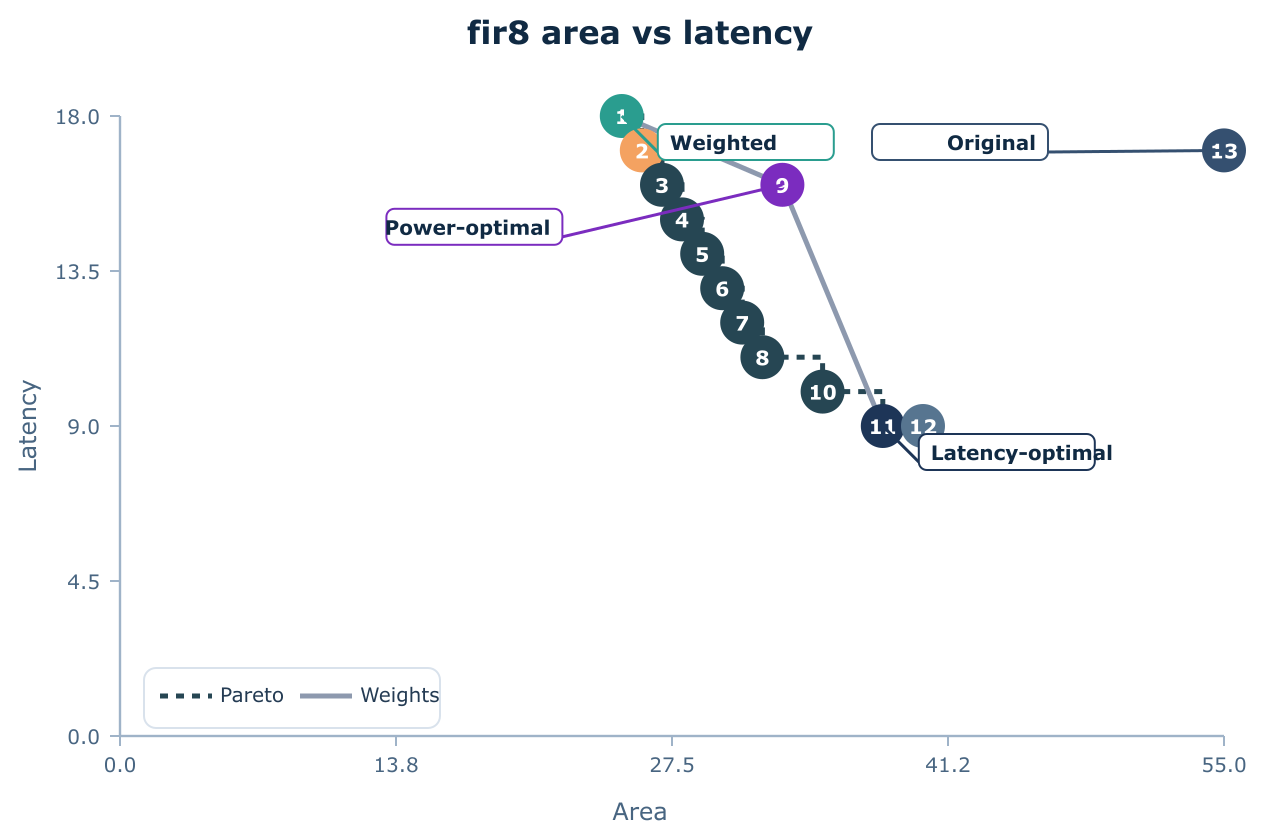
\includegraphics[width=\columnwidth]{figures/fir8_tradeoff.png}
\caption{Representative \texttt{fir8} area--latency tradeoff. The weighted, latency-optimal, and power-proxy-optimal points occupy distinct locations on the retained frontier. Their full $A/L/P/D/U$ totals are shown in Table~\ref{tab:main-results}.}
\label{fig:fir8-tradeoff}
\end{figure}

Figure~\ref{fig:fir8-tradeoff} and Table~\ref{tab:main-results} show that the added extraction modes change the selected design. On \texttt{fir8}, the weighted point, latency-optimal point, and power-proxy-optimal point are all different; none dominates the others across analytical area, analytical latency, and normalized power proxy simultaneously. The same kind of separation appears across the suite. Latency-optimal extraction improves analytical latency by 41.7\% on average relative to baseline, and exact Pareto extraction still exposes 10.5 nondominated area--latency points per benchmark on average. The retained design space is therefore not degenerate under this model. The power-proxy objective remains secondary: it helps most clearly on \texttt{fir8} and \texttt{conv3x3}, but it is less reliable on kernels such as \texttt{dot16}, which is expected because the metric is only an analytical proxy. This shows that the project's main contribution is not just generating equivalences, but selecting different implementations from the same e-graph under different objectives.

The per-benchmark behavior reinforces that interpretation: \texttt{fir8} exposes a middle power-proxy point, the GEMM and \texttt{stencil5} cases often return the baseline as the best power-proxy choice, and \texttt{conv3x3} improves on the original graph in several ways.

\subsection{Q3: Do Constraints Reveal Meaningful Boundaries of the Design Space?}
Table~\ref{tab:main-results} summarizes how much the constrained queries change the answer relative to default weighted extraction. Most `min Lat $|$ Area cap' and `min Lat $|$ Power cap' queries improve their target metric substantially, which shows that explicit budgets are doing real filtering rather than being checked after the fact. The strongest negative result is \texttt{dot16}: both `min Lat $|$ Power cap' and `min Lat $|$ LUT cap' are infeasible. This is useful evidence, not a failure of presentation. It means the extractor respects the budgets instead of always returning a superficially different answer. The result is that constraints reveal real boundaries of the design space, which is the key difference from SEER's equivalence-generation story.

The resource-oriented queries also show what kind of alternatives the retained frontier contains. The zero-DSP query remains feasible across the suite, but it predictably pushes the selected points toward slower LUT-only datapaths. That is the expected behavior for a hard resource budget. Conversely, the LUT-capped query either recovers a more DSP-heavy implementation or fails outright. This contrast matters because the system is not merely toggling operator labels. It is selecting among implementations with different binding patterns and exposing when those patterns do or do not fit the requested budget.

\subsection{RTL and Quartus Validation}
The analytical results also correspond to generated datapaths, not only different scores attached to an abstract expression. The RTL exporter generates Verilog variants for each feasible extraction result. ModelSim checks each benchmark on 200 deterministic signed 32-bit vectors; every testbench computes an independent golden result from the benchmark definition, checks the original RTL, and then checks every feasible non-original variant against the same result. All 29 non-original variants pass.

\begin{table}[t]
\caption{Representative RTL/Quartus resource-steering evidence on multiplier-heavy kernels. DSP and ALM are post-fit Quartus resources; Fmax is the reported STA estimate, not a timing-signoff claim. These rows show that LUT-multiplier variants trade DSP blocks for ALMs; they do not establish global optimality or measured power.}
\label{tab:quartus-validation}
\centering
\scriptsize
\setlength{\tabcolsep}{2.5pt}
\resizebox{\columnwidth}{!}{%
\begin{tabular}{@{}l l r r r@{}}
\toprule
Benchmark/variant & Mapping & DSP & ALM & Fmax \\
\midrule
\texttt{dot16} orig. & DSP & 24 & 732 & 166.69 \\
\texttt{dot16} soft & LUT mult. & 0 & 4328 & 186.78 \\
\texttt{gemm\_k8} orig. & DSP & 12 & 366 & 190.95 \\
\texttt{gemm\_k8} soft & LUT mult. & 0 & 2154 & 245.16 \\
\texttt{gemm\_blocked} orig. & DSP & 12 & 366 & 190.95 \\
\texttt{gemm\_blocked} soft & LUT mult. & 0 & 2154 & 245.16 \\
\bottomrule
\end{tabular}
}
\end{table}

Quartus compiles all 35 generated variants. Table~\ref{tab:quartus-validation} gives the clearest backend evidence: on \texttt{dot16} and the GEMM kernels, soft/LUT-multiplier variants reduce fitted DSP usage to zero, at the expected cost of substantially higher ALM usage, and they also change reported Fmax. Fmax is a backend timing estimate, not proof that latency-minimizing analytical selections are universally faster. Smaller kernels are less informative because Quartus legally optimizes, merges, and remaps equivalent arithmetic into identical fitted resources. Thus, the FPGA result supports a narrow claim: constrained extraction can steer backend resource usage on multiplier-heavy datapaths. It does not show consistent post-fit latency, Fmax, or total-area improvement for every generated variant, and it does not validate the analytical power proxy.

\section{Discussion}
\begin{sloppypar}
Relative to SEER, the project demonstrates one concrete point: equality saturation is a good way to generate HLS datapath alternatives, but constrained extraction is what makes those alternatives usable. The results are strongest where the weighted point is clearly not the right answer and where explicit budgets either recover a better implementation or expose infeasibility. That is why the negative \texttt{dot16} cases are useful rather than a weakness: they show that the extractor reports when a requested budget cannot be met.

The takeaway is simple: constrained extraction changes how an e-graph is used. In SEER, equality saturation is primarily an optimization substrate. Here, the same saturated graph is also a queryable design-space representation: one run can answer latency, area, normalized power proxy, and feasibility questions under different budgets. That is why the constrained interface is more than a small change to cost-based extraction.
\end{sloppypar}

\section{Limitations}
\begin{sloppypar}
The scope prevents broader claims. The IR is datapath-only: there is no frontend, MLIR or CIRCT integration, control flow, or memory/BRAM model. The cost model is analytical, so the reported numbers are controlled relative comparisons rather than device-accurate performance or energy predictions. Quartus is also an optimizing synthesis tool, not a literal Verilog interpreter. Even with resource-style attributes, it can simplify small datapaths and map distinct source expressions to the same fitted circuit. Fully preventing that behavior would require lower-level primitive instantiation, which is outside this prototype.

The C++/\texttt{i++} path is similarly limited: it confirms HLS-frontend acceptance, but it is not primary evidence because Intel HLS estimates collapse most variants to identical resource reports.

There are four main threats to validity. First, the bounded frontier may discard useful candidates, so the results describe the retained design space rather than the full theoretical equivalence space. Second, budgets are analytical, not fitted FPGA limits; feasibility means ``under this model,'' not ``for every device.'' Third, the power-proxy objective distinguishes operator classes and resource bindings, but it does not model switching activity, placement, routing, or clocking effects. Fourth, RTL validation is simulation-based rather than formal, and the Quartus evidence comes from one Arria 10 flow. These limitations matter for external fidelity, but not for the internal comparison because every extraction mode uses the same model.
\end{sloppypar}

\section{Future Work}
The next steps are direct continuations of the proposal: import kernels from C, MLIR, or CIRCT; add memory/BRAM-aware constraints; and calibrate the analytical area, latency, and normalized power proxies against larger synthesis-report corpora. These extensions test whether the same constrained interface remains useful with a richer frontend and a physical backend.

\section{Conclusion}
This report presents a constrained-extraction extension of the SEER idea for HLS-style arithmetic kernels. SEER establishes that equality saturation can generate equivalent datapaths; this project shows that explicit objectives and budgets can change which implementation should be selected from that space. In the evaluated kernels, default weighted extraction is often not sufficient, constrained objectives recover different operating points, and some budget combinations are genuinely infeasible. The main lesson is that an e-graph is more useful for HLS when it can answer constrained design questions and expose feasibility boundaries, not only return one scalar-cost expression.


\clearpage
\bibliographystyle{ACM-Reference-Format}
\bibliography{references}

\end{document}
